\documentclass[12pt]{article}
\usepackage[T2A]{fontenc}
\usepackage[utf8]{inputenc}
\usepackage[russian]{babel}
\usepackage{graphicx, float, hyperref}

\begin{document}
    \begin{titlepage}
        \begin{center}
            \vspace*{1cm}

            \Huge
            \textbf{Закон всемирного тяготения.\\Точки Лагранжа}

            \vspace{1.5cm}

            \Large
            \textbf{Балдин Виктор Б01-303}

            \vfill

            Вопрос по выбору \\
            Устный экзамен по общей физике

            \vspace{0.8cm}

            
\includegraphics[width=0.4\textwidth]{university_logo.png}

            Физтех-школа радиотехники и компьютерных технологий\\
            Московский физико-технический институт\\
            Долгопрудный, 2024
        \end{center}
    \end{titlepage}

    \begin{abstract}
        \par Данный вопрос по выбору включает в себя теоретические расчеты
        положения точек Лагранжа и обсуждение некоторых их интересных
        свойств. В работе используются материалы из различных открытых
        источников об истории исследований на эту тему и современном их
        состоянии.
        \par Точки Лагранжа являются крайне важным объектом для изучения
        космического пространства в современной астрофизике.
        В частности, прямым образом их свойства используются для размещения
        космических аппаратов, предназначенных для наблюдений дальнего
        космоса.
        \par Автор выражает надежду, что данный вопрос по выбору содержит
        актуальные сведения и благодарит экзаменационную комиссию за его
        рассмотрение.
    \end{abstract}

    \newpage

    \section{Введение}
    \par \textbf{Точки Лагранжа}, в некоторых источниках также \textbf{точки
    либрации} или \textbf{L-точки} -- точки в системе двух тел, в которых
    третье тело может оставаться неподвижным относительно первых двух.
    \par Нахождение точек Лагранжа является частным случаем решения задачи
    трех тел для случая круговых орбит и малой массы одного из них. То есть,
    другими словами, два массивных тела равномерно вращаются вокруг общего
    центра масс. В этой ситуации существует 5 точек, в которых третье
    невесомое (обладающее пренебрежимо малой массой) тело может оставаться
    неподвижным в системе отсчета, связанной с массивными телами.
    \par Точки Лагранжа названы в честь математика Жозефа Луи Лагранжа,
    который первым в 1772 году показал их существование.
    \begin{figure}[H]
        \centering
        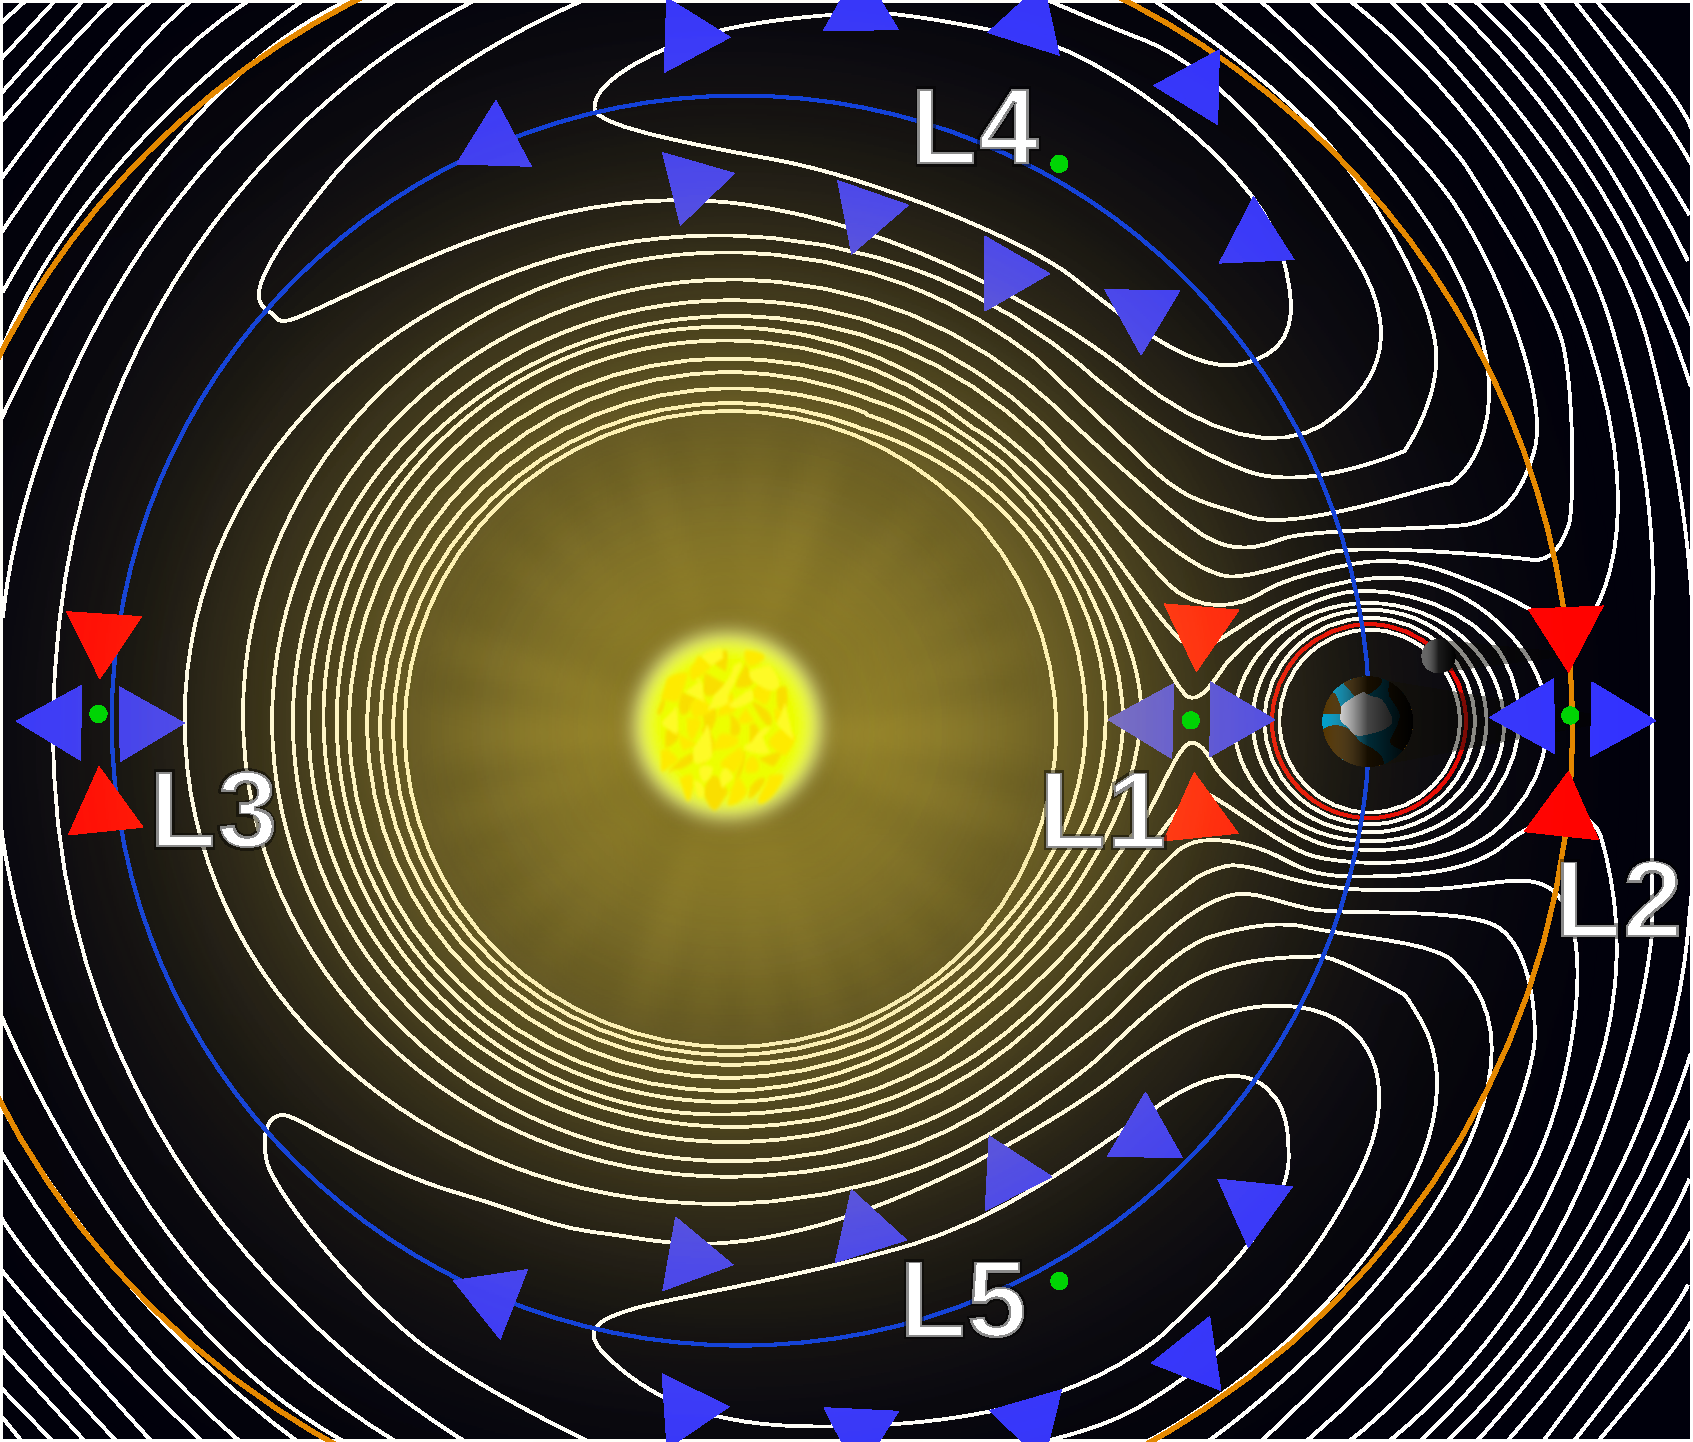
\includegraphics[scale=0.35]{Lagrange_points.pdf}
        \caption{5 точек Лагранжа и гравитационные эквипотенциальные
        поверхности системы двух тел\\
        \textbf{Источник:}
        \url{https://upload.wikimedia.org/wikipedia/commons/thumb/e/ee/
        Lagrange_points2.svg/1920px-Lagrange_points2.svg.png}}
    \end{figure}

\end{document}

